\documentclass{article}

\usepackage{explorations}
\usepackage{longtable}

\lesson{1.1.2.2 --- Introduction to Rational Numbers}

\newcommand{\numrow}[1]{\ensuremath{#1} & & My justification: \newline \vspace{0.1in} \newline Other number sets?\newline \vspace{0.1in}\\ \hline}

\usepackage[none]{hyphenat}

\begin{document}

The ancient Greeks initially thought all numbers were rational numbers. That is, they could be represented as the ratio, or quotient, or two integers. Now it is known that there are other numbers which are not rational numbers.

\begin{dfn}
  A \emph{rational number} is a number that can be written as the ratio of two integers.
\end{dfn}

Preliminary Questions

\begin{enumerate}
\item What is a ratio?

  \vfill
  
\item What does terminating mean?

  \vfill
  
\item Give examples of words in the English language that have the same root as the verb to terminate.

  \vfill
  
\item Give at least two examples of a terminating decimal.

  \vfill
  
\item Give at least two examples of a non-terminating decimal.

  \vfill
  
\item Give at least two examples of a non-terminating, repeating decimal.

  \vfill

  \clearpage
  
\item Give at least two examples of a non-terminating, non-repeating decimal.

  \vfill
  
\item Give examples of three rational numbers. Write one as a decimal, write one as a fraction, and one as an integer.

  \vfill
  
\item Is the sum of two rational numbers always rational?? Justify your answer.

  \vfill
  
\item A student enters in her calculator. She sees the following screen. Can the student determine if is rational by looking at the screen? What if she had a calculator that showed to 20 decimal places? Discuss the limitations of a calculator when displaying integers, rational numbers, and irrational numbers.

  \begin{figure*}[h!]
    \centering
    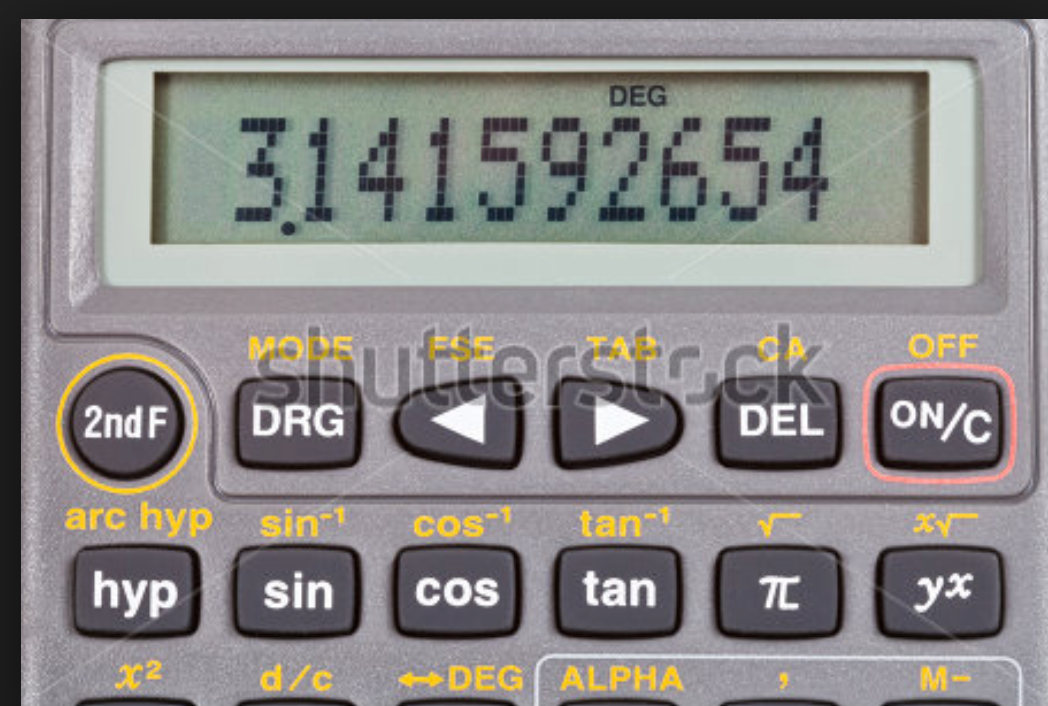
\includegraphics[width=0.4\textwidth]{calculator.png}
  \end{figure*}

  \vfill
  
\item How many rational numbers are there on the real number line? Give your reasoning.

  \vfill

  \clearpage
  
\item How many rational numbers are there on the real number line that are greater than 0 and less than 1? Give your reasoning.

  \vspace{1in}
  
\item After completing by yourself the following table, interchange your table with your partner and make comments on each item on the table.
\end{enumerate}
\begin{center}
  \rowcolors{2}{gray!25}{white}
  \begin{longtable}{|>{\centering\arraybackslash} m{1in}|>{\centering\arraybackslash} m{0.6in}|m{4.7in}|}
    \hline \rowcolor{gray!50} \textbf{Number} & \textbf{Is this a rational number?} & \textbf{Justify your answer and have your neighbor comment on your
      justification.} \\ \hline
    \endhead
    \numrow{7}
    \numrow{\displaystyle\frac59}
    \numrow{\sqrt{7}}
    \numrow{\displaystyle-\frac17}
    \numrow{0}
    \numrow{\displaystyle\frac04}
    \numrow{0.12\overline{3}}
    \numrow{\displaystyle\frac{22}{7}}
    \numrow{0.125}
    \numrow{0.\overline{125}}
    \numrow{3\%}
    \numrow{\displaystyle\frac{\sqrt{3}}{2}}
    \numrow{\sqrt{25}}
    \numrow{\sqrt{7}}
    \numrow{400\%}
    \numrow{0.333}
    \numrow{\scriptstyle\left(\sqrt{5}-2\right)\left(\sqrt{5}+2\right)}
    \numrow{0.\overline{3}}
    \numrow{\pi}
    \numrow{2.718281828}
  \end{longtable}
\end{center}
\begin{enumerate}[resume]
\item The diagram below represents the real number system. Based on the diagram can you write 3 sentences that describe the relationship between natural numbers, whole numbers, integers, rational numbers and irrational numbers. For example: Any whole number is an integer.

  \begin{figure*}[h!]
    \centering
    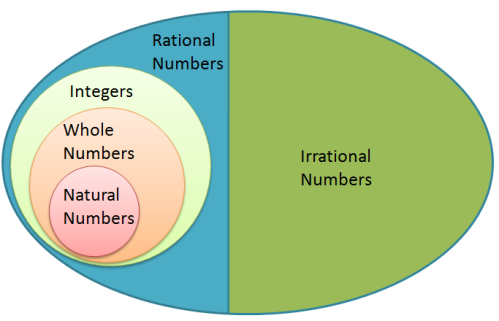
\includegraphics[width=0.4\textwidth]{diagram.png}
  \end{figure*}
\end{enumerate}

\end{document}

%%% Local Variables:
%%% mode: latex
%%% TeX-master: t
%%% End:
